% TODO: Choose thesis language.
\documentclass[estonian,english]{unitartucs-thesis} % Thesis is in English, but info page also has Estonian.
% \documentclass[english,estonian]{unitartucs-thesis} % Thesis is in Estonian, but info page also has English.

% Modern encoding, do not remove.
\usepackage[utf8]{inputenc}
\usepackage[T1]{fontenc}

% Bibliography with BibLaTeX.
% TODO: Choose citation and bibliography style.
\usepackage[style=unitartucs-numeric]{biblatex} % Numeric citations [1], alphabetically sorted bibliography.
% \usepackage[style=unitartucs-numeric,sorting=none]{biblatex} % Numeric citations [1], bibliography in citation order.
% \usepackage[style=unitartucs-alphabetic]{biblatex} % Alphabetic citations [ABC], alphabetically sorted bibliography.

\DeclareLanguageMapping{english}{unitartucs-english} % Language overrides for english.
\DeclareLanguageMapping{estonian}{unitartucs-estonian} % Language overrides for estonian.
\addbibresource{thesis.bib} % Bibliography file itself.

% Packages for math.
\usepackage{amsmath}
\usepackage{amssymb} % Package for additional math symbols.
\usepackage{amsthm} % Package for theorems, definitions, etc.
\theoremstyle{plain}
\newtheorem{theorem}{Theorem} % TODO: Translate to Teoreem if thesis is in Estonian.
\theoremstyle{definition}
\newtheorem{definition}{Definition} % TODO: Translate to Definitsioon if thesis is in Estonian.

% Package for graphics/images.
\usepackage{graphicx}
\graphicspath{{figures/}} % Directory of graphics.

\usepackage{booktabs} % Package for nice and professional tables (\toprule, \midrule, \bottomrule).
\usepackage{subcaption} % Package for subfigures and subtables.

% Package for source code.
\usepackage{minted}
\setminted{autogobble} % Trim common leading whitespace from code.

\usepackage{xspace} % Non-eatable spaces in macros
% Define your favorite macros that you use inside the thesis
% Name followed by non-removable space
\newcommand{\proveit}{ProveIt\xspace}

% Macros that make sure that the math mode is set
\newcommand{\typeF}[1] {\ensuremath{\mathsf{type_{#1}}}\xspace}
\newcommand{\opDiv}{\ensuremath{\backslash \mathsf{div}}\xspace}
\newcommand{\typeInt}{\ensuremath{\mathsf{Int}}\xspace}

% Package for TODO notes with \todo command.
\usepackage{todonotes}
\newcommand{\TODO}{\todo[inline]} % Custom command for inline TODOs.


% TODO: Fill in title and author name.
\title{Type Inference for Fourth Order Logic Formulae}
\author{Alice Cooper}

% TODO: Fill in supervisors. Use \and to separate multiple supervisors. Use \degree to specify their degree.
\supervisor{Axel Rose\degree{MSc} \and May Flower\degree{PhD}}

% TODO: Choose curriculum.
\curriculum{Computer Science Curriculum}
% \curriculum{Software Engineering Curriculum}
% \curriculum{Informaatika õppekava}

% TODO: Choose thesis type (bachelor's or master's) and number of ECTS.
\thesis{Master's Thesis (30 ECTS)}
% \thesis{Bakalaureusetöö (9 EAP)}
% \thesis{Bachelor's Thesis (9 ECTS)}

% Override year (on title page) and date (in licence). Defaults to today.
% \date{2023-01-02}


\appto\biburlsetup{\Urlmuskip=0mu\relax} % https://tex.stackexchange.com/a/291857
\begin{document}

\maketitle % Title page
\newpage
\pdfbookmark[section]{\infoname}{info} % Add info page to PDF bookmarks (for convenience), but not to Table of Contents.

% Info in main language.
\begin{info}
\begin{abstract}
% TODO: Add abstract.
Many interpreting program languages are dynamically typed, such as Visual Basic or Python. As a result, it is easy to write programs that crash due to mismatches of provided and expected data types.  One possible solution to this problem is automatic type derivation during compilation. In this work, we consider study how to detect type errors in the \textsc{Whitespace} language by using fourth-order logic formulae as annotations. The main result of this thesis is a new triple-exponential type inference algorithm for the fourth-order logic formulae. This is a significant advancement as the question of whether there exists such an algorithm was an open question.
All previous attempts to solve the problem lead to logical inconsistencies or require tedious user interaction in terms of interpretative dance. Although the resulting algorithm is slightly inefficient, it can be used to detect obscure programming bugs in the \textsc{Whitespace} language. The latter significantly improves productivity. Our practical experiments showed that productivity is comparable to average Java programmer.
From a theoretical viewpoint, the result is only a small advancement in a rigorous treatment of higher-order logic formulae. The results obtained by us do not generalise to formulae with the fifth or higher order.
\end{abstract}

% TODO: Add keywords, separated by commas.
\keywords{\TODO{List of keywords}}

\cercs{\TODO{CERCS code and name:~\url{https://www.etis.ee/Portal/Classifiers/Details/d3717f7b-bec8-4cd9-8ea4-c89cd56ca46e}}}
\end{info}


% Info in other language.
% TODO: Choose other language (estonian or english).
% TODO: Fill in title in other language.
\begin{otherinfo}{estonian}{Tüübituletus neljandat järku loogikavalemitele}
\begin{abstract}
% TODO: Add abstract in other language.
\TODO{One or two sentences providing a basic introduction to the field, comprehensible to a scientist in
any discipline.}
\TODO{Two to three sentences of
more detailed background, comprehensible to scientists in related disciplines.}
\TODO{One sentence clearly stating the general problem being addressed by this particular
study.}
\TODO{One sentence summarising the main result (with the words ``here we show´´ or their equivalent).}
\TODO{Two or three sentences explaining what
the main result reveals in direct
comparison to what was thought to be the case previously, or how the main result adds to previous knowledge.}
\TODO{One or two sentences to put the results into a more general context.}
\TODO{Two or three sentences to provide a
broader perspective, readily
comprehensible to a scientist in any
discipline, may be included in the first paragraph
if the editor considers that the accessibility of
the paper is significantly enhanced by their inclusion.}
\end{abstract}

% TODO: Add keywords in other language, separated by commas.
\keywords{\TODO{List of keywords}}

\cercs{\TODO{CERCS kood ja nimetus:~\url{https://www.etis.ee/Portal/Classifiers/Details/d3717f7b-bec8-4cd9-8ea4-c89cd56ca46e}}}
\end{otherinfo}
 % Info page

% Table of Contents
\newpage
\pdfbookmark[section]{\contentsname}{toc} % Add Table of Contents to PDF bookmarks (for convenience), but not to Table of Contents itself.
\tableofcontents

% TODO: Uncomment if you want a list of remaining TODOs. Remove from final version!
% \newpage
% \listoftodos

\newpage
\section{Introduction}

\TODO{What is it in simple terms (title)?}
\TODO{Why should anyone care?}
\TODO{What was my contribution?}
\TODO{What you are doing in each section (a sentence or two per section)}

Tip: if it's hard for you to start writing, then try to split it into smaller parts, e.g., if the title is ``Type Inference for a Cryptographic Protocol Prover Tool'' then the ``What is it'' can be divided into ``what is type inference'', ``what is cryptographic protocol'' and ``what is the prover tool''. These three can also be split into smaller parts etc.






\subsection{How to use references} \label{sec:using_ref}

\paragraph{Cross-references to figures, tables, and other document elements.}
LaTeX  internally numbers all kinds of objects that have sequence numbers:
\begin{itemize}
\item chapters, sections, subsections;
\item figures, tables, algorithms;
\item equations, equation arrays.
\end{itemize}
To reference them automatically, you have to generate a label using \texttt{$\backslash$label\{some-name\}} just after the object that has the number inside. Usually, labels of different objects are split into different namespaces by adding a dedicated prefix, such as \texttt{sec:}, \texttt{fig:}. To use the corresponding reference, you must use command \texttt{$\backslash$ref} or \texttt{$\backslash$eqref}. For instance, we can reference this subsection by calling Section~\ref{sec:using_ref}. Note that there should be a nonbreakable space \texttt{\~} between the name of the object and the reference so that they would not appear on different lines (does not work in Estonian).



\paragraph{Citations.}
Usually, you also want to reference articles, webpages, tools or programs, or books. For that, you should use citations and references. The system is similar to the cross-referencing system in LaTeX. For each reference, you must assign a unique label. Again, there are many naming schemes for labels. However, as you have a short document, anything works. To reference to a particular source you must use \texttt{$\backslash$cite\{label\}} or \texttt{$\backslash$cite[page]\{label\}}.

References themselves can be part of a LaTeX source file. For that, you need to define a bibliography section. However, this approach is really uncommon. It is much easier to use BibTeX to synthesise the right reference form for you. For that, you must use two commands in the LaTeX source:
\begin{itemize}
\item $\backslash$bibliographystyle\{alpha\} or $\backslash$bibliographystyle\{plain\}
\item $\backslash$bibliography\{file-name\}
\end{itemize}
The first command determines whether the references are numbered by letter-number combinations or by cryptic numbers. It is more common to use \texttt{alpha} style. The second command determines the file containing the bibliographic entries. The file should end with \texttt{bib} extension. Each reference there is in a specific form. The simplest way to avoid all technicalities is to use graphical frontend  Jabref (\url{http://jabref.sourceforge.net/}) to manage references. Another alternative is to use the DBLP database of references and copy BibTeX entries directly from there.


The following paragraph shows how references can be used. Game-based proving is a way to analyse the security of a cryptographic protocol~\cite{GameB_1, GameB_2}. There are automatic provers, such as {CertiCrypt\-}~\cite{certiCrypt} and ProVerif~\cite{proVerif}.

\section{How to add figures and pictures to your thesis}


Here are a few examples of how to add figures or pictures to your thesis (see Figures~\ref{fig:fnCompModel}, \ref{fig:game-based_proofs}, \ref{fig:proveit_screenshot}).

Rule: All the figures, tables and extras in the thesis have to be referred to somewhere in the text.


\begin{figure} [ht] %try to place the figure here (next option top of the page)
\begin{center}
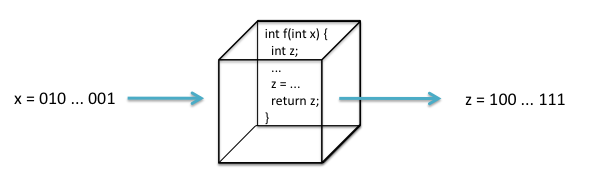
\includegraphics[width=0.8\textwidth]{computational_model_function}
\caption{The title of the Figure.}
\label{fig:fnCompModel}
\end{center}
\end{figure}



\begin{figure} [!ht] %if [h] doesn't work, we can force with !
\begin{center}
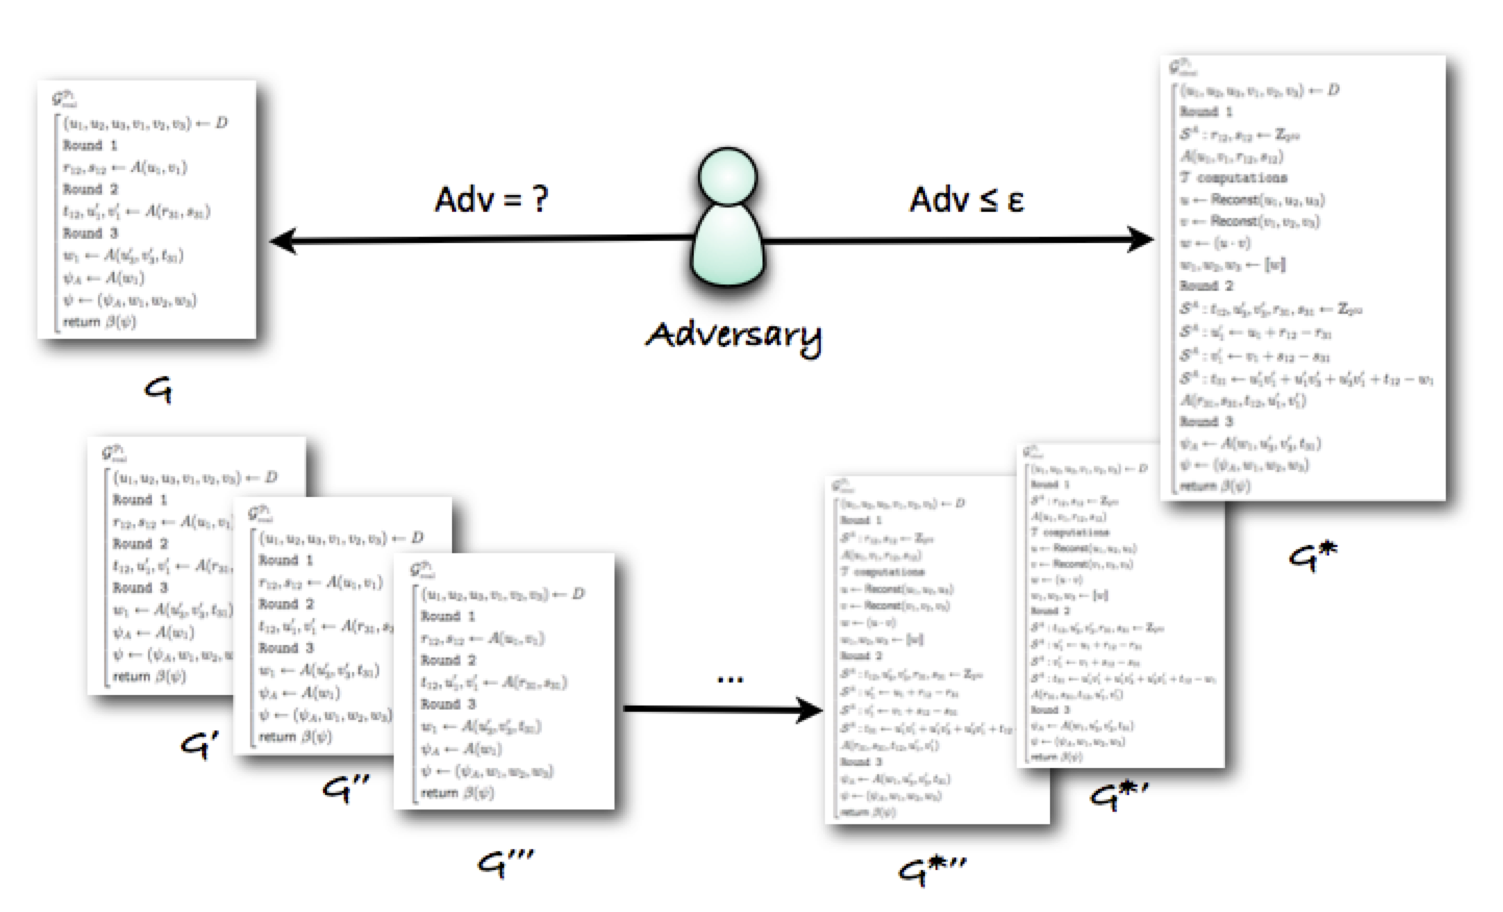
\includegraphics[width=\textwidth]{game-based_proofs}
\caption{Refer if the figure is not yours~\cite{kamm12}.}
\label{fig:game-based_proofs}
\end{center}
\end{figure}


\begin{figure} [p]
\begin{center}
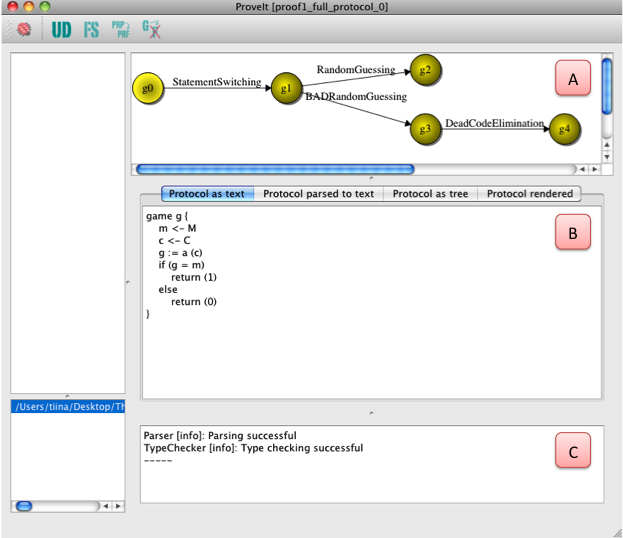
\includegraphics[width=\textwidth]{proveit_screenshot}
\caption{Screenshot of \proveit.}
\label{fig:proveit_screenshot}
\end{center}
\end{figure}

Tip: If you add a screenshot, then labeling the parts might help make the text more understandable (panel C vs bottom left part), e.g.


\begin{figure} [htbp]
  \centering
\begin{subfigure}{0.45\textwidth}
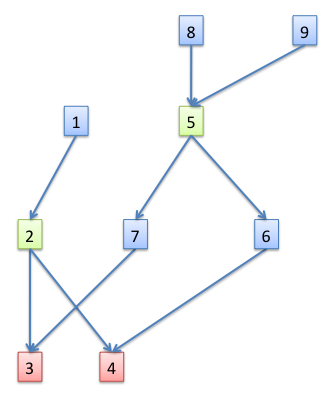
\includegraphics[width=\textwidth]{LCA_2_solutions}
\caption{Example graph.}
\end{subfigure}
\hfil
% TODO: mixing subfigure and subtable in figure is odd
\begin{subtable}{0.3\textwidth}
\centering
\caption{Descendants per node.}
\begin{tabular}{cl}
  \toprule
	Node & Decendants \\
  \midrule
  1 & 2, 3, 4 \\
  2 & 3, 4 \\
  3 & \\
  4 & \\
  5 & 3, 4, 6, 7 \\
  6 & 4 \\
  7 & 3 \\
  8 & 3, 4, 5, 6, 7\\
  9 & 3, 4, 5, 6, 7\\
  \bottomrule
\end{tabular}
\end{subtable}
%
\caption{Example how to put two figures parallel to each other.}
\label{fig:LCA_2_solutions}
\end{figure}


Example: A screenshot of \proveit can be seen in Figure~\ref{fig:proveit_screenshot}. The user first enters the pseudocode of the initial game in panel B. \proveit also keeps track of all the previous games showing the progress on a graph seen in panel A.

There are two figures side by side in Figure~\ref{fig:LCA_2_solutions}.

\section{Other Ways to Represent Data}

\subsection{Tables}

\begin{table}[h]
\centering
\caption{Statements in the \proveit language.}
\begin{tabular}{ll}
	\toprule
	Statement & Typeset Example \\
	\midrule
	assignment & $a := 5 + b$ \\
	uniform choice & $m <- M$ \\
	function signature & $f : K \times M -> L$ \\
	\bottomrule
\end{tabular}
\label{tab:statements}
\end{table}


\subsection{Lists}

Numbered list example:
\begin{enumerate}
	\item item one;
	\item item two;
	\item item three.
\end{enumerate}

\subsection{Math mode}
Example:
\begin{equation}
a + b = c + d
\end{equation}
Aligning:
\begin{align*}
	a &= 5 \\
	b + c &= a \\
	a -2*3 &= 5/4
\end{align*}
Hint: Variables or equations in text are separated with \$ sign, e.g. $a$, $x - y$.


\subsection{algorithm2e}

\begin{algorithm} [!h]
	\caption{typeChecking} \label{alg:typeChecking}
	\KwIn{Abstract syntax tree}
	\KwResult{Type checking result; In addition, type table \typeF{type\_G} for global variables, \typeF{game} for the main game and \typeF{fun} for each $fun \in F$}
	\SetKwData{s}{s}
	\BlankLine

	\While{something changed in last cycle}{
		\lForEach{global statement \s} {
			\parseStatement{\s, \typeF{type\_G}}\;
		}
		\ForEach{function $fun$} {
		\lForEach{statement \s in $fun$} {
			\parseStatement{\s, \typeF{fun}}\;
		}
		}
		\lForEach{statement \s in game} {
			\parseStatement{\s, \typeF{game}}\;
		}
	}
	%\eIf{error messages were found}{\Return \False\;}{\Return \True\;}
\end{algorithm}

\subsection{Pseudocode}

\begin{figure} [htb]
\begin{lstlisting}
expression
  : NUMBER
  | VARIABLE
  | '+' expression
  | expression '+' expression
  | expression '*' expression
  | function_name '(' parameters ')'
  | '(' expression ')'
\end{lstlisting}
\caption{Grammar of arithmetic expressions.}
\label{fig:parser_exp}
\end{figure}

\subsection{Frame Around Information}

Tip: We can use minipage to create a frame around some important information.
\begin{figure} [h]
\frame{
\begin{minipage}{\textwidth}
\begin{enumerate}
	\item integer division ($\opDiv$) -- only usable between \typeInt types
	\item remainder ($\%$) -- only usable between \typeInt types
\end{enumerate}
\end{minipage}
}
\caption{Arithmetic operations in \proveit revisited.}
\label{fig:aritmOp_revisit}
\end{figure}

\section{Conclusion}

\TODO{what did you do?}
\TODO{What are the results?}
\TODO{future work?}


% Bibliography
\clearpage % Flush all floats (figures and tables) before bibliography and start new page.
\nocite{*}
\printbibliography[heading=bibintoc] % Bibliography with heading also in Table of Contents.

% Appendices
\newpage
\begin{appendices}

\section{Glossary}
\label{app:glossary}

\printlicence % Licence

\end{appendices}

\end{document}
